% Drawing 87/02-1 -- folder 87, batch 02, archive page 29 (PDF page 30).
% Transcription: à gauche, un petit croquis : quatre segments issus d'un point, dans un cercle, deux d'entre eux repassés à l'encre
% Kind: segments from a point inside a circle. Method 2 (schematic redraw from the facsimile). Status: partial.
% Notes: From a heavy central point, two strokes inked thick (up left, up right) and three thinner ones (down left, down, down right); around the point a thin irregular closed outline (the circle, drawn as a polygon) and two short strokes. Five segments are visible from the point where the transcription says four (noted).
% Coordinates: 1 unit = 1 mm = 1/100 of the crop width (bbox in page fractions: [0.19, 0.69, 0.28, 0.75]).
% Redrawn by Claude (claude-opus-5-5), issue #73, 2026-11-07; not checked by a human; not compiled (no TeX in the session).
% Rights: reproduces part of the work -- behind RENDER_TRANSCRIPTS, never published by itself.
\documentclass[tikz,border=3pt]{standalone}
\usepackage{amsmath,amssymb}
\usetikzlibrary{patterns,arrows.meta}
\tikzset{pencil/.style={black!45}, struck/.style={black!35}, mark/.style={circle,draw,inner sep=1.3pt}, pt/.style={circle,fill,inner sep=0.9pt}, opt/.style={circle,draw,fill=white,inner sep=1.1pt}}
\begin{document}
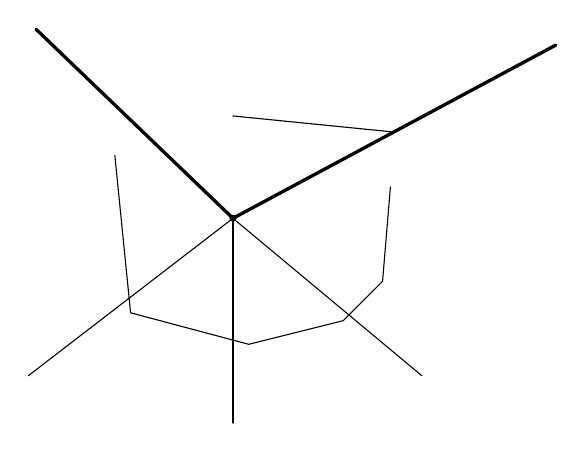
\begin{tikzpicture}[x=1mm,y=1mm,line cap=round,line join=round,font=\scriptsize]
\draw[very thick] (50,-44) -- (25,-20);
\draw[very thick] (50,-44) -- (91,-22);
\node[pt] at (50,-44) {};
\draw (50,-44) -- (24,-64);
\draw (50,-44) -- (50,-70);
\draw (50,-44) -- (74,-64);
\draw (35,-36) -- (37,-56) -- (52,-60) -- (64,-57) -- (69,-52) -- (70,-40);
\draw (50,-31) -- (70,-33);
\end{tikzpicture}
\end{document}
